% chapter2.tex (Literature Review)

\chapter{Literature Review}
\label{ch:litrev}

The aim of the literature review is to introduce the problem domain. This chapter gives background information on the existing work in the field, noting the research most important and relevant to this project. It outlines the study into the connections between network flow problems and their related problems in graph theory, and suggests areas for expansion on the surveyed literature.

\section{Traditional Routing}
\label{sect:routing}

Traditional routing involves choosing paths in a network for data transmission. It treats messages sent along the network as packets, which cannot be divided into smaller units, or otherwise altered. This method is used in a large variety of real-world networking applications, such as traffic management, telephone networks and computer networks.

Routing may be controlled manually by configuring specific routing tables to direct packets along the most direct route, or in a more autonomous manner by assigning certain routing protocols allowing the packets more freedom in the route taken. These different methods of forwarding information are known as schemes (Figure~\ref{fig:routing_schemes}), and vary in techniques --- from delivering the information to one specific node, to delivering the information to all adjacent nodes regardless of whether they requested it.

Unicast (Figure~\ref{unicast}) is the most common routing scheme used in current telecommunications networks. It involves the sending of the packets to exactly one destination. Broadcasting (Figure~\ref{broadcast}) is the opposite of unicasting; the packets are forwarded to every node in the network. Multicasting (Figure~\ref{multicast}) is a more sophisticated approach, similar to broadcasting. In multicasting, packets are sent to a number of adjacent nodes determined by some calculation of a minimum spanning tree. Anycasting (Figure~\ref{anycast}) is slightly different in that it has a number of possible nodes to which it may forward the packet, but only one node is ultimately chosen to receive it.

\begin{figure}[ht]
     \centering
     \subfigure[]{
          \label{unicast}
          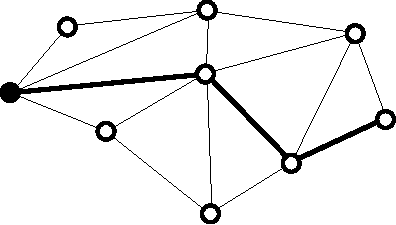
\includegraphics[width=.4\textwidth]{figures/unicast.pdf}}
     \hspace{.3in}
     \subfigure[]{
          \label{broadcast}
          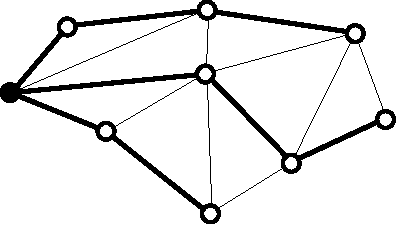
\includegraphics[width=.4\textwidth]{figures/broadcast.pdf}} \\
          
     \subfigure[]{
          \label{multicast}
          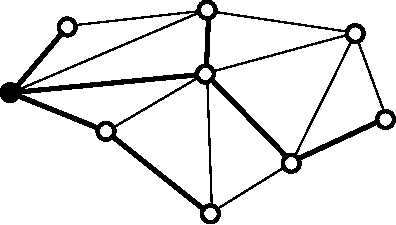
\includegraphics[width=.4\textwidth]{figures/multicast.pdf}}
     \hspace{.3in}
     \subfigure[]{
          \label{anycast}
          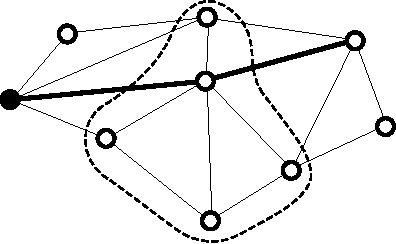
\includegraphics[width=.4\textwidth]{figures/anycast.pdf}}

		 \label{fig:routing_schemes}
		 \caption[Some network routing schemes used for packet forwarding]{Examples of the different schemes used in packet forwarding: \subref{unicast} unicast, \subref{broadcast} broadcast, \subref{multicast} multicast and \subref{anycast} anycast. Packets are forwarded from the black node along the bold edges.}
\end{figure}

Network routing is an enourmously successful data transmission method, seen by its use in so many existing technologies. However, its methods may limit the transfer rate in certain cases --- for instance, bottlenecks may appear in certain network topologies. These may be due to the fact that information is viewed as a discrete unit, something which may not be broken down into smaller components. This is akin to viewing the atom as the building-block of the universe; whilst it was once viewed as the most advanced model, technology showed that it was possible to break it down into yet smaller components, and that different combinations of these components yielded different atoms. To eliminate these bottlenecks, a similar paradigm shift was required.

\section{Network Coding}
\label{sect:netcod}

As mentioned above, traditional routing is used in a number of information networks, from communication in a processor to communication across the Internet. However, there are disadvantages to using these techniques; a simple network can be constructed where no routing method can achieve optimal flow.

\begin{figure}[ht]
	\centering
	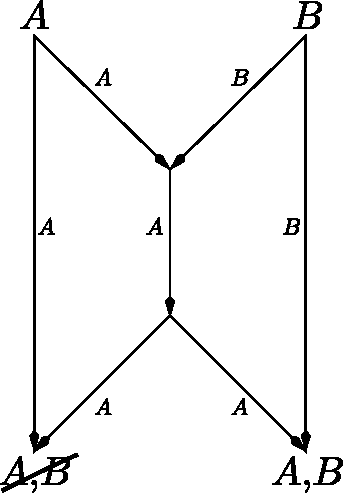
\includegraphics[width=100pt]{figures/butterfly.pdf}
	\caption[The butterfly network using routing]{The butterfly network, first introduced by Ahlswede \textit{et al.} \cite{ahls2000}. Because of the central bottleneck, routing is insufficient: the left sink node fails to resolve both $A$ and $B$.}
	\label{butterfly}
\end{figure}

In the so-called ``butterfly'' network in Figure~\ref{butterfly}, first introduced in \cite{ahls2000}, the two sink nodes at the bottom each need to receive both messages $A$ and $B$ from the two source nodes at the top. The edges between each vertex denote paths or channels along which data may flow, and the arrows signify the direction in which it may travel. Assume that each channel can transmit only one message per unit time. If traditional routing is used, then only trivial functions may be used. This means that the middle channel cannot transmit both $A$ and $B$ at the same time, resulting in a bottleneck. If the central channel transmits only $A$, then the left sink node does not resolve both messages. If this particular network set-up appeared in a real-world situation, for instance client computers requesting information from two separate servers, then one client would be forced to wait until all the information had been transmitted to the other client before completing its own requests.

\textbf{Network coding} is an emerging field of information theory in which messages are viewed as information. This means that any node in the network may replicate or alter the messages. In other words, the outgoing edges from a given node will transmit some function of the data received on the incoming edges. For instance, if on the network in Figure~\ref{butterfly} the exclusive disjunction $A \oplus B$ is sent along the middle channel, the sink nodes can resolve both messages (Figure~\ref{butterfly-netcod}). To see this, node that the left sink node receives $A$ from the left source node, and $A \oplus B$ from the central channel. Since $A \oplus B \oplus A = B$, it is possible to compute both original messages $A$ and $B$, as desired. The process is similar for the right sink node.

\begin{figure}[ht]
	\centering
	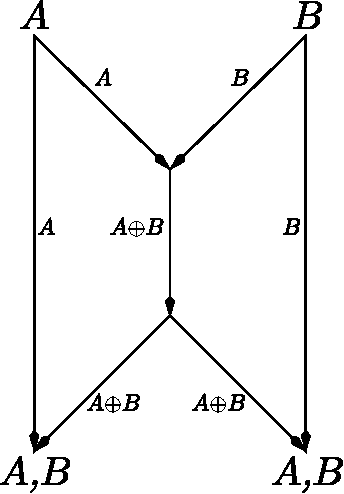
\includegraphics[width=100pt]{figures/butterfly-netcod.pdf}
	\caption[The butterfly network using network coding]{Using network coding allows both sources to successfully resolve both messages.}
	\label{butterfly-netcod}
\end{figure}

In this manner, the entire method of traditional routing can be viewed as the trivial case of network coding when only the trivial functions are used; in other words, the output of each function is equal to one of its inputs.

\newpage

In general, if the message $m_{x, y} = f(x, y) \in A$ (for some finite alphabet $A$) is sent along the middle channel, then the problem can be solved if and only if $f(x, y)$ is a Latin function \cite{riah2004}.\footnote{The function $f(x, y)$ is Latin if for each $(x, y) \in A^2$, the functions $m_y : A \rightarrow A : x \mapsto m_y(x) = f(x, y)$ and $n_x : A \rightarrow A : y \mapsto n_x(y) = f(x, y)$ are bijective maps.} The main aim of using network coding is to find a set $F$ of such functions, called a \emph{solution}, to allow all of the sink nodes to be satisfied. The network is said to be \emph{solvable} if $F$ exists.

If a solution uses only trivial functions it is known as a \emph{routing solution}, and if (as in the butterfly network) the output of each function is a linear combination of its inputs, it is known as a \emph{linear solution} \cite{cann2006}. To refine these definitions even further, if the messages passed along the nodes are scalar quantities, then a solution is known as a \emph{scalar linear solution}. Often, however, it is useful to consider message vectors, or blocks of scalar messages; in this case, a solution is called a \emph{vector linear solution}.

The problem of the butterfly network above can be converted into a problem in graph theory by representing the network as a circuit, and identifying nodes. Such a representation is called \emph{circuit representation}. Converting the networks in this manner allows all of the tools at the disposal of the graph theorist to be used on problems in network coding. In this representation, all of the computations in the network are carried out in the nodes. Circuit representation is a slightly different (but mathematically equivalent) representation of a network coding problem which serves to be a slightly more useful (if less accurate) method of depicting the network coding problem \cite{riis2005util}. A source node $s$ is identified with the output node(s) (or sink nodes with respect to $s$) attempting to compute the information transmitted from $s$. This particular problem results in $K_3$, or the complete graph on $3$ nodes \cite{riis2005util}. The proof of this conversion is illustrated in Figure~\ref{butterfly_to_k3}. The motivation behind this conversion is to have an equivalent problem that can be expressed in graph theoretic terms \cite{riis2005util, riis2005info}.

\begin{figure}[ht]
	\centering
	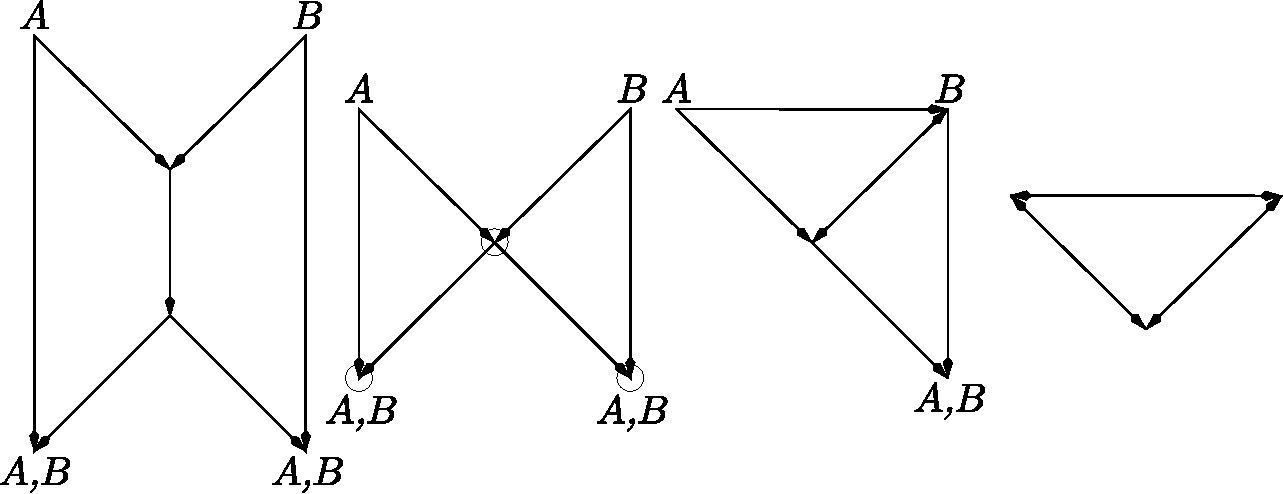
\includegraphics[width=350pt]{figures/butterfly_to_k3.pdf}
	\caption[Converting the butterfly network to a graph]{Start with Figure~\ref{butterfly}. First, the network is represented as a circuit information flow problem, with computation at the nodes. Then the sink nodes are identified with the source nodes, resulting in $K_3$.}
	\label{butterfly_to_k3}
\end{figure}

Network coding has shown its usefulness in a number of areas for concern; one important example is its improvements to wireless networking. Increases in throughput and energy efficiency are evident in wireless network topologies as well as other networks \cite{sagd2005}. With wireless access points becoming so popular, and with their limited range requiring intermediate access points or mesh networks, there is growing concern for the security of data broadcast via radio waves. Network coding has been shown to be a useful approach to prevent eavesdropping on secure communications \cite{caiy2002}. As mentioned above, information theory is primarily concerned with transmission of data over noisy channels, and network coding has been shown to be a successful alternative to other error-correction methods \cite{lars2006}.

Network coding has also been considered for peer-to-peer (P2P) content distribution, and is even believed by some that it may improve performance over P2P networks, but Chiu \textit{et al.} conclude that there is little or no coding advantage, due in part to the time and resources required to decode the delivered information \cite{chiu2006}.

\subsection{Linear versus Non-Linear Coding}
\label{sect:lin_v_nonlin}

Previously, it has been conjectured by a number of authors (for example, \cite{meda2003, bary2006}) that linear network coding is optimal for an arbitrary network topology. Indeed it is known that every solvable multicast network does have a scalar linear solution provided the alphabet is a sufficiently large finite field \cite{liye2003}. Moreover, any solvable multicast network has a linear solution in some vector dimension \cite{riis2004}. However, it is also known that this result does not extend to arbitrary networks (see, for instance, \cite{lehm2003}). Dougherty \textit{et al.} \cite{doug2005} provide a solvable network that does not have a linear solution over any finite field, or indeed over any module.\footnote{A module is a concept in abstract algebra that generalises the idea of a vector space. The notion of a vector space being expressed over a field is also generalised; a module is expressed over a ring.} Riis and Ahlswede introduce other counter-examples, but suggest that these are so far only ``rare isolated incidences'' \cite{riah2004}.

\section{Guessing Numbers}
\label{sect:guessing_number}

The concept of a \textbf{guessing number} was developed by S{\o}ren Riis \cite{riis2005util, riis2005info} to investigate the solutions of particular network flow problems. The concept was notably used to provide a counter-example \cite{riis2005info} to the conjectures made by Leslie Valiant \cite{vali1975}. To understand the meaning of the guessing number of a graph, consider the following problem:

Imagine a game consisting of $n$ players, each of whom has an $s$-sided die (for $s \in \NN$, $s > 1$), where each side is labelled in the usual manner from $1$ through to $s$.\footnote{In accordance with most papers in computer science, the set $\NN$ of natural numbers is defined as the non-negative integers, that is $\NN = \{ n \in \ZZ : n \geq 0 \}$.} The dice are rolled simultaneously in such a way that no player knows the value of their own die. The task for the players is to guess the value of their own die.

\begin{enumerate}
	\item What is the probability that all $n$ players can correctly guess their die value?
	
	\item Now assume that each player knows the value of every die except their own. What is the probability that they all guess correctly now?
\end{enumerate}

In the first question, each player acts independently and, since the probability that each player is right is $1/s$, all $n$ players guess correctly with probability $s^{-n}$. 

At first glance, it may seem that allowing the players to see the other players' dice cannot improve their odds, since the information held on other dice in no way alters the value of one's own die. However, the players may adopt a ``strategy'' that uses the information provided to them from the others. There are many strategies that the players may adopt to utilise this information, but the best (or \emph{optimal}) strategy is for the players to assume beforehand that the sum of all the dice is congruent to $a$ modulo $s$. The player then calculates the sum total of the other dice, $T$, and ``guesses'' their value to be $a - T$ modulo $s$. Clearly if the result is $0$, then the player must guess $s$, since no side is labelled $0$. This strategy ensures that all players ``guess'' the value of their own die with probability $1/s$ if (and only if) one player guesses correctly. Note that since any one player can only guess correctly with probability $1/s$, this gives an upper bound on the guessing number, and hence this is an optimal strategy.

The game (or class of games) mentioned above is a subclass of a larger class of co-operative games, known as guessing games. A guessing game is a method of representing a problem from $\mathcal{C}_{mu}$, the class of multiple-unicast information flow problems \cite{riis2005util}. A multiple-unicast problem is a network with $n$ source nodes $\{i_r\}$ and $n$ sink nodes $\{o_r\}$, where each output node $o_r$ must resolve the message $m_r$ from the corresponding input node $i_r$. The game is played on a directed graph $G = (V, E)$ where $V$ is the set of vertices, and $E \subseteq V^2$ the set of edges between those vertices. In the case of a directed graph, there is an edge from $v \in V$ to $w \in V$ if and only if $(v, w) \in E$ --- in other words, $E$ is a collection of ordered pairs.\footnote{In the undirected case, $E$ is a collection of unordered pairs, or sets of cardinality $2$; an undirected edge between $v$ and $w$ is denoted $\{v, w\}$.} Each vertex represents a player in the game, and edges represent communication paths between the players. If the graph is directed, then the communication may only travel along the edge in one direction, for instance from the head to the tail. Note that all graphs in this class are simple, in that they do not contain any self-loops. In the game, a self-loop would correspond to a player immediately and explicitly knowing the value of their die once thrown.

\newpage

\begin{definition}[Riis \cite{riis2005util}]

A \emph{guessing game}, denoted $\mathrm{GuessingGame}(G, s)$, is played as follows: each player $v \in V$ is randomly assigned a value $m_v \in A$, where $A = \{1, 2, \dots, s\}$. The players then communicate their values to adjacent players, i.e. to all players $w$ with $(v, w) \in E$. Node $w$ receives a set of values $M_w = \{m_v \in A : (v, w) \in E\}$. From the information received, each player must resolve their own value. Assuming that the players have agreed on a strategy, the probability that all players guess correctly can be calculated. Explicitly, a \emph{strategy} or \emph{protocol} is a set of functions $f_w : A^{|M_w|} \rightarrow A$ for each $w \in V$. A function $f_w$ denotes player $w$'s guess.

\end{definition}

There are very many co-operative strategies for the players to adopt: in general, there are $s^{\sum _{v \in V} {s^{|M_v|}}}$ strategies. Each strategy has associated with it a probability determining the likelihood of success of that strategy. Clearly the strategy that yields the maximum probability is optimal.

The alphabet $A$ from which the values are assigned need not be as simple a structure as described above; it could, for instance, be a field, a ring, or (as was used in one proof in \cite{riis2005util}) a commutative group; suitable algebraic structures must include some notion of linearity. However, for most cases the description provided above is adequate.

Just like the butterfly network considered previously, the example guessing game corresponds to a complete graph; every player is connected by an edge to every other player. Therefore, the total number of guessing strategies available to the players of this game is $s^{ns^{n - 1}}$. As shown above, the optimal strategy for players in this situation gives a probability of success of $1/s$, a factor $s^{n - 1}$ better than uncoordinated, random guessing. This gives us a \emph{guessing number} of $n - 1$, the exponent of the quotient of the probabilities.

The formal definition of the guessing number of a graph is as follows:

\begin{definition}[Riis \cite{riis2005util}]

Let $G = (V, E)$ be a graph where each vertex $v \in V$ corresponds to a player of the guessing game. $G$ has \emph{guessing number} $k = k(G, s)$ if there is a strategy that ensures their success with probability $s^{k - |V|}$. In other words, the strategy succeeds with probability $s^k$ times higher than independent, random guessing.

\end{definition}

The guessing number is often independent of $s$. Also, rather surprisingly, for many graphs the guessing number is also an integer. Though it is noted in \cite{riis2005util} that there exists a directed graph where the guessing number depends on $s$, it is left as an open question as to whether the guessing number of an undirected graph is always an integer. Later, in Chapter~\ref{ch:sol}, it is shown that there exists an undirected graph where the guessing number depends on $s$ and is never an integer.

The guessing game $G_N$ can be said to be a graph representation of a specific information network (or subclass of networks) $N \in \mathcal{C}_{mu}$. The mathematically correct representation of the network is called ``standard representation''. In this representation (and throughout this thesis) a network $N$ is a directed acyclic multi-graph, where source nodes have in-degree $0$, and sink nodes have out-degree $0$. Each source node $i_r$ is associated with exactly one message $m_r \in \Gamma_{var}$ (this notation is used for consistency with \cite{riis2005util}). Each outgoing edge from a given node $v$ transmits the same function $f_v : A^d \rightarrow A$, where $d$ is the in-degree of $v$. Each sink node needs to resolve some subset of the variables in $\Gamma_{var}$.

The standard representation of the circuit information flow problem $N$ is converted to the directed graph $G_N$ by introducing a vertex for each variable or function assigned to an edge or node in $N$, and identifying each input node $i_r$ with its corresponding output node $o_r$ for each $r \in \{1, 2, \dots, n\}$.

If the guessing game has some meaning in information flow problems, then it is reasonable to assume that the guessing number has a similar generalisation. Before this generalisation is explained, some definitions are required.

\begin{definition}[Riis \cite{riis2005util}]

The \emph{global success rate} of $N$ with respect to a set of coding functions $F$ is the probability that all outputs correctly determine their messages, given that the inputs are selected randomly from a finite alphabet $A$ and with independent probability distribution. It is denoted $p(N, s, F)$ where $s = |A|$.

\newpage

The \emph{maximum global success rate} $p(N, s)$ is the supremum of all global success rates $p(N, s, F)$ for any choice of coding functions $F$. Since the set of functions $F$ is finite, $p(N, s) = p(N, s, F)$ for some $F$.

\end{definition}

\begin{definition}[Riis \cite{riis2005util}]

The \emph{source transmission bandwidth} of the information network $N$ over alphabet $A$ is defined as $k(N, s) = \log_s(p(N, s)) + n$, where $n$ is the number of source nodes of $N$.

\end{definition}
%%%%%%%%%%%%%%%%%%%%%%%%%%%
This definition generalises the concept of a guessing number \cite{riis2005util}. The guessing strategies used in the guessing game correspond exactly to the network coding functions in the network flow problem.

As proved in \cite{riis2005info}, a network flow problem $N$ with $n$ input/output nodes has a solution over alphabet $A$ with $|A| = s$ elements if and only if the corresponding graph $G_N$ has guessing number $k(G_N, s) \geq n$.

In \cite{riis2005util}, it was shown that if a network $N'$ appears from a network $N$ by application of $r$ split moves and $t$ inverse split moves, and $N$ has global success rate $p$, then $N'$ has global success rate $ps^{t - r}$. A ``split move'' is a simple operation applied to an inner (not an input or output) node $w \in V$ in a network $N = (V, E)$. The operation copies the node $w$, creating two nodes $w_{\mathrm{input}}$ and $w_{\mathrm{output}}$. Explicitly, $\mathrm{split} : \mathcal{C}_{mu} \rightarrow \mathcal{C}_{mu} : N \mapsto N'$ where $N' = (V', E')$, $V' = V \cup \{ w_{\mathrm{input}}, w_{\mathrm{output}} \} \setminus \{ w \}$ and $E'$ contains all the edges of $E$ except those connecting to $w$, plus $(w, u) \in E \Rightarrow (w_{\mathrm{input}}, u) \in E'$ and $(u, w) \in E \Rightarrow (u, w_{\mathrm{output}}) \in E'$, each counted with multiplicities. Since the split and inverse split moves are applied only to the inner nodes of $N$, in other words those nodes in $V \setminus \{i_1, i_2, \dots, i_n, o_1, o_2, \dots, o_n \}$, the source transmission bandwidth remains unchanged under them, and hence $k(N, s) = k(N', s)$.

It is worth noting that if $N'$ can be realised from $N$ by applying a certain number of split and/or inverse split moves, then the graphs $G_N$ and $G_{N'}$ are identical. This is because creating the graph $G_N$ is effectively the same as applying as many inverse split moves as possible to $N$. In other words, $G_N$ is invariant under split moves on $N$.

\section{Routing Capacity}
\label{sect:routing_capacity}

Although the messages transmitted in a network are scalar quantities, it can be useful to consider blocks of these quantities as vectors. If the capacity of each edge in the network is of the same dimension as these message vectors, then any vector solution corresponds directly to a scalar solution where the alphabet consists of vectors. \emph{Fractional coding} refers to the case where edges vectors and message vectors differ in dimension.

Cannons \textit{et al.} \cite{cann2006} look at fractional coding for networks in the case of routing, referred to as \emph{fractional routing}. The \textbf{routing capacity} $\epsilon$ of a network is ``the supremum of all possible fractional message throughputs achievable by routing'' \cite{cann2006}. In other words, it is the highest possible ratio of message dimension to edge capacity that can be obtained using a fractional routing solution. A \emph{$(k, n)$ fractional routing solution} is a solution where message vectors are of dimension $k$ and edges have capacity $n$. Routing capacity is essentially a method brought about by the failure of other methods to provide the best possible data transmission for certain networks, and it is this advantage over linear network coding that will be exploited in Chapter~\ref{ch:sol}.

The routing capacity of every network was shown to be both achievable and rational \cite{cann2006}. Furthermore, it is shown that for each $r \in \QQ$, $r > 0$, there exists a network whose routing capacity is equal to $r$, and that any $r \in (0, 1] \cap \QQ$ is the routing capacity of a solvable network. The concept of routing capacity is generalised to \emph{coding capacity}, with the inferred definition. The coding capacity of a network is proven to be independent of the underlying alphabet.

\begin{figure}[ht]
	\centering
	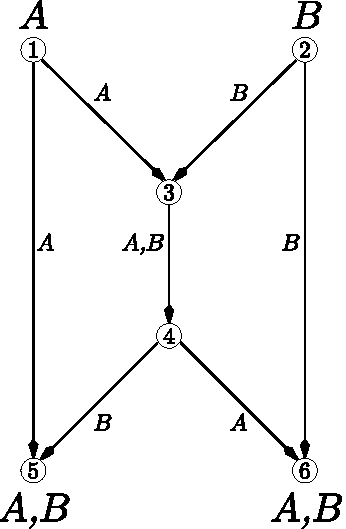
\includegraphics[width=100pt]{figures/butterfly-routing.pdf}
	\caption[Routing capacity of the butterfly network]{The butterfly network, which has been shown to have a linear coding solution, has routing capacity $1/2$.}
	\label{butterfly-routing}
\end{figure}

The butterfly network in Figure~\ref{butterfly-netcod} was shown to have a linear coding solution, namely if the central channel transmits the function $A \oplus B$. In Figure~\ref{butterfly-routing}, if both $A$ and $B$ are to be transmitted along the central edge $(3, 4)$, the edge capacity $n$ must be at least twice the vector dimension $k$, hence $2k \leq n$ and $\epsilon = k/n \leq 1/2$. Now by transmitting $A$ along edges $(1, 3)$, $(1, 5)$ and $(4, 6)$, $B$ along edges $(2, 3)$, $(2, 6)$ and $(4, 5)$, and transmitting $(A, B)$ along $(3, 4)$, there is a fractional routing solution to the network, and $\epsilon \geq 1/2$. From above, the routing capacity of the butterfly network is $\epsilon = 1/2$ \cite{cann2006}.

A slightly more complicated example of routing capacity is the network $\mathcal{N}$ shown in Figure~\ref{routing}. In \cite{doug2005}, it was shown that $\mathcal{N}$ has no linear solution for any vector dimension over a finite field with odd cardinality (it was shown in the same paper, however, that it has a scalar linear solution over any ring of cardinality $2$). The three messages $A$, $B$ and $C$ are transmitted by $1$, $2$ and $3$ respectively, and are demanded by $14$, $13$ and $12$ respectively. The following proof is reproduced from \cite{cann2006}, and shows that the $\mathcal{N}$ has a coding solution with routing capacity $2/3$.

The edges $(1, 12)$, $(3, 9)$ and $(7, 14)$ can be immediately ignored, since none of the edges can transmit any useful information to their sink nodes. For example, node $7$ receives information about the messages $B$ and $C$, but node $14$ is only concerned with message $A$. Ignoring these edges implies that $(4, 6)$ and $(5, 7)$ carry all the information from the sources to the sinks. Since there are $3$ messages to be transmitted along $2$ edges, this quickly imposes an upper bound of $\epsilon = 2/3$ as $3k \leq 2n$ for any $k, n$. Now let $(k, n) = (2, 3)$ --- so message have $2$ components and edges have capacity $3$ --- and transmit the messages as follows:

\begin{eqnarray*}
  	(1, 4) = (11, 14) & = & (A_1, A_2) \\
  	(2, 4) = (11, 13) & = & (B_1) \\
  	(2, 5) = (10, 13) & = & (B_2) \\
  	(3, 5) = (10, 12) & = & (C_1, C_2) \\
  	(4, 6) = (6, 9)   & = & (A_1, A_2, B_1) \\
  	(5, 7) = (7, 8)   & = & (B_2, C_1, C_2)
\end{eqnarray*}

\begin{figure}[ht]
	\centering
	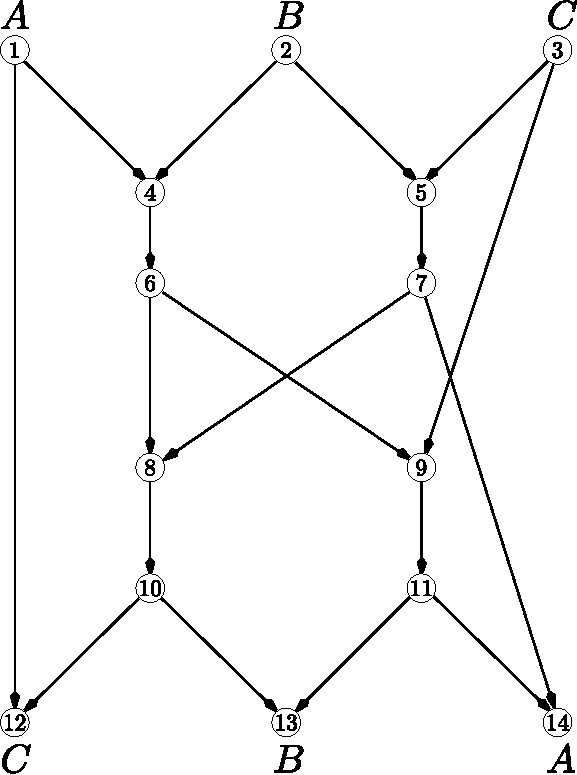
\includegraphics[width=180pt]{figures/routing.pdf}
	\caption[Routing capacity of the network $\mathcal{N}$]{The network $\mathcal{N}$, reproduced from \cite{cann2006}, has routing capacity $2/3$.}
	\label{routing}
\end{figure}

This gives a fractional routing solution to $\mathcal{N}$, meaning $\epsilon \geq 2/3$ and hence $\epsilon = 2/3$. Note that when omitting the ignored edges together with $(6, 8)$ (which also remains unused), we obtain a satisfyingly bisymmetric subgraph of $\mathcal{N}$, which goes some way to explain the symmetry of the routing solution.

As mentioned in Chapter~\ref{ch:intro}, even though a number of questions are answered in \cite{cann2006}, some questions are left open; for instance, whether the coding capacity is achievable for every network, and if algorithms exist for computing the coding capacity of a network. It has since been shown that the coding capacity of an arbitrary network is not always achievable by the network, unlike the case of routing capacity \cite{doug2006}.

\section{Information Entropy}
\label{sect:entropy}

Shannon's classical information inequalities \cite{shan1948} will be used to calculate the guessing numbers of cycles in Chapter~\ref{ch:sol}. Shannon's inequalities are a number of rules governing \textbf{information entropy} $H(X)$, the measure of uncertainty of a particular random variable.
%%%%%%%%%%%%%%%%%%%%%%%%%%%
\begin{eqnarray*}
  	H(X) & = & \mathrm{E}(I(X)) \\
	       & = & \quad \sum_{i = 1}^n p(x_i) \, \log_2 \, ( 1 / p(x_i)) \\
	       & = & - \sum_{i = 1}^n p(x_i) \, \log_2 \, (p(x_i))
\end{eqnarray*}
%%%%%%%%%%%%%%%%%%%%%%%%%%%
Here, $I(X)$ is the self-information of $X$, or the information associated with the outcome of $X$, and $p(x_i) = \Pr(X \! = \! x_i)$. In the same manner, entropy can be thought of as the amount of self-information that is missing when the value of $X$ is unknown.

A fundamental result in information entropy is Gibbs' inequality; that is,

$$
	\sum p_i \log_2 \, p_i \geq \sum p_i \log_2 \, q_i
$$

for probability vectors $P = (p_1, \dots, p_n)$, $Q = (q_1, \dots, q_n)$.

\begin{figure}[ht]
	\centering
	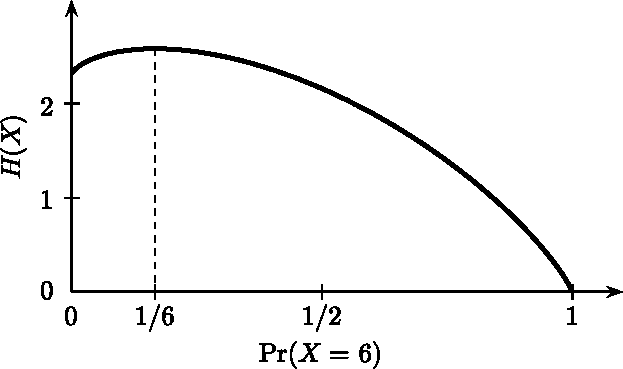
\includegraphics[width=250pt]{figures/weighted_die.pdf}
	\caption[Graph showing entropy of a weighted die]{The graph of entropy shows that less information is provided when the probability of rolling a $6$ approaches $1$. The entropy function is maximised when the probability of throwing a $6$ is $1/6$, where the die is fairest.}
	\label{weighted_die}
\end{figure}

A simple example would be a weighted die that can be altered to offer bias to different outcomes (Figure~\ref{weighted_die}). The more bias toward a certain outcome, the less uncertainty there is in the result of the roll. If the die is weighted such that every roll produces a $6$, say, then the roll provides no information, and the entropy of the outcome is $0$. If the dice has no bias, then the uncertainty is maximised, and the entropy is $\log_2 6 \approx 2.58$. When logs are taken to base $2$, entropy is measured in bits. In the case of statistical information, a ``bit'' is slightly different from the storage unit used in digital computers. In digital storage, a bit is a discrete quantity taking only one of the values in $\{0, 1\}$. In terms of entropy, a variable with $n$ bits of information can theoretically, and on average, be stored on a computer using $n$ bits, though this value is a minimum. The value indicates the number of bits of actual information contained in the result, and as such provides a lower bound on any lossless compression of the data. 

This can be explained by the notion of ``redundancy''. Ordinary text in the English language has a great redundancy --- certain phonemes or letters that are not strictly required to convey the original message. Take, for example, an advertisement for training in shorthand notation: ``\emph{f u cn rd ths msg u cn hv a hi pyng jb}'' \cite{glei1990}. Compare also with telex speak and SMS language, where similar shorthand is used to convey the message in the limited number of characters available. If, as with ASCII encoding, each letter has an entropy of exactly $7$ bits when chosen at random, English text has an entropy of between $1$ and $1.5$ bits per letter; it is quite easy to determine the next letter in the sequence \cite{schn1996}. This exact principle can be used in cryptography to break simple substitution ciphers, by working out the frequency of appearance of each letter.

\section{Bipartite Graphs}
\label{sect:bipartite}

It is possible to rearrange problems in network flow to a bipartite flow problem. In this arrangement, there are two copies of each node, one copy having the same in-degree as the original node, and the other having the same out-degree as the original node. This is the result of applying the split move mentioned in Section~\ref{sect:guessing_number} to \emph{all} inner nodes in a graph $N$ to get the bipartite graph $B_N$ with no inner nodes \cite{riis2005util}. The result is shown in Figure~\ref{fig:bipartite}, where the the edges are implicitly directed from top to bottom. As mentioned above, the two are different representations of mathematically equivalent problems.

\begin{figure}[ht]
     \centering
     \subfigure[Network flow problem]{
          \label{fig:pre-bipartite}
          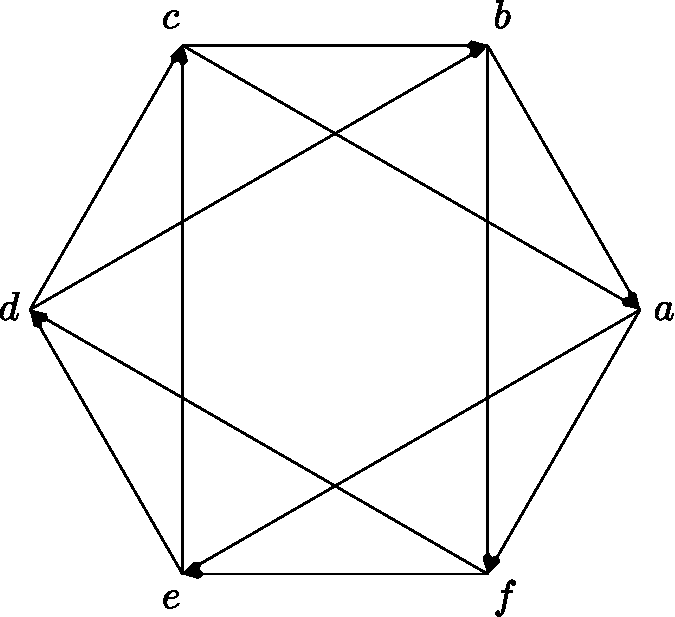
\includegraphics[height=.35\textwidth]{figures/pre-bipartite.pdf}}
     \hspace{.3in}
     \subfigure[Equivalent bipartite flow problem]{
          \label{fig:bipartite}
          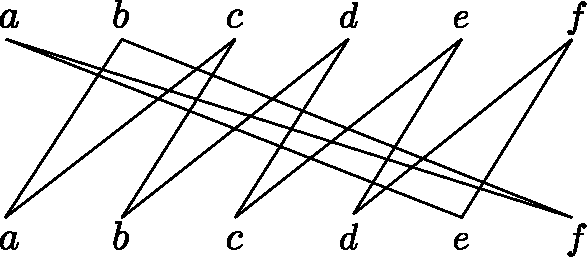
\includegraphics[width=.45\textwidth]{figures/bipartite.pdf}}

		 \caption[Rearranging a graph into a bipartite flow problem]{The graph in \subref{fig:pre-bipartite} is converted to the bipartite problem in \subref{fig:bipartite} by making two copies of each node.}
\end{figure}

Bipartite graphs are the heart of a different game introduced in the same paper as the guessing game, known as $\mathrm{PublicChannelGame}(G, P)$. In this game, each node has access to a number of public messages $p \in P$, $p : A^n \rightarrow A$ as well as all the messages received from its own incoming vertices. In the case of a guessing game, it is always possible to substitute a suitable public channel for the guessing part of the game if and only if the solution is linear \cite{riis2005util}.

\section{Matchings and Fractional Matchings}

A \emph{matching} $M$ of an undirected graph $G$ is a subset of the edges $E$ of $G$ such that no two edges in $M$ share a common vertex (Figure~\ref{fig:matching}). A \emph{perfect matching} is a matching that covers every node in the graph (Figure~\ref{fig:perfect}).

\begin{figure}[ht]
     \centering
     \subfigure[]{
          \label{fig:matching}
          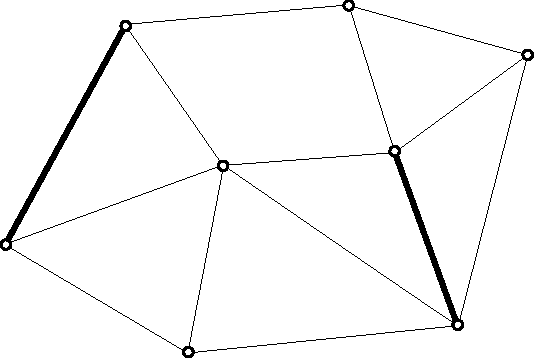
\includegraphics[width=.45\textwidth]{figures/matching.pdf}}
     \hspace{.3in}
     \subfigure[]{
          \label{fig:perfect}
          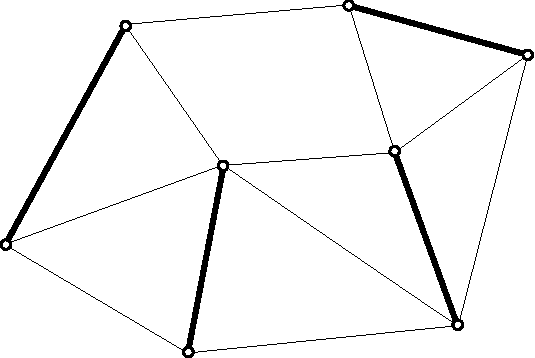
\includegraphics[width=.45\textwidth]{figures/perfect_matching.pdf}}
     \caption[Matching and perfect matching on a graph]{A matching (marked by bold lines) \subref{fig:matching} is a set of pairwise non-adjacent edges, and a perfect matching \subref{fig:perfect} is a matching that covers all the vertices.}
\end{figure}

A fractional matching of a graph $G$ is a function $f : E \rightarrow [0, 1]$ such that for any $u \in V$, $\sum_{v \, : \, \{ u, v \} \, \in \, E} f( \{ u, v \} ) \leq 1$ \cite{liuy2002}. The \emph{fractional matching number} of a graph is the supremum of all fractional matchings, $\sup \sum_{ \{ u, v \} \, \in \, E} f( \{ u, v \} )$.

A \emph{perfect fractional matching} is observed when each of the sums is exactly equal to $1$. As with matchings, fractional matchings only apply to undirected graphs. Here, the weightings refer to the capacities of the vertices.

\section{The Fractional Matching Problem}

The Fractional Matching Problem is a well-known problem in graph theory:
%%%%%%%%%%%%%%%%%%%%%5
\begin{eqnarray*}
  \mbox{Maximise} && \sum_{e \in E} x_e \\
  \mbox{such that} && \forall v \in V \sum_{e \ni v} x_e \leq 1 \\
  && x_e \geq 0.
\end{eqnarray*}

The above problem has been stated in many forms. It was shown by Bourjolly and Pulleyblank (see, e.g., \cite{bour1989}) that there exists a maximum solution to the fractional matching problem that is half-integral, with each edge having a capacity in $\{0, \frac{1}{2}, 1 \}$. The theorem is stated below. The proof is outlined in two stages and follows from Theorem~\ref{thm:pul}.

\begin{theorem}
  For every graph, there exists a fractional matching that is half-integral, where each edge in the matching has its weighting in $\{0, \frac{1}{2}, 1 \}$.
\end{theorem}

Let $G(V, E)$ be a graph, and denote by $c_e \in \RR$ the weighting assigned to the edge $e \in E$. Denote by $c = (c_e: e \in E)$ the vector of these edge weights.

For each edge $e$, define a variable $x_e \in \{ 0, 1 \}$. Now denote by $x^J$ the incidence vector representing $J \in E$, where

$$
x_e^J = \left\{ \begin{array}{rl}
 0 &\mbox{ if $e \notin J$,} \\
 1 &\mbox{ if $e \in J$.}
\end{array} \right.
$$

Let $\RR^E$ be the set of all real-valued vectors indexed by $E$. Let $x(J) = \sum{ (x_j : j \in J) }$ for any $J \subseteq E, x \in \RR^E$. Let $\mathcal{M} = \{ x^M \in \RR^E \}$, where $M$ is a perfect matching in $G$. $\mathcal{M}$ is a (finite) set of $(0, 1)$-valued vectors, the convex hull of which is a polytope\footnote{A \emph{polytope} is the generalisation of a polygon in two dimensions, a polyhedron in three dimensions, and so on. A \emph{convex hull} for a set $X$ is the minimal convex set containing $X$.} in $\RR^E$. It is called the \emph{perfect matching polytope}, and is denoted $PM(G)$. 

Since every polytope is the solution set of a finite system of linear equalities \cite{weyl1935}, we attempt to find such a system for $PM(G)$.

\begin{theorem}[{Edmonds \cite{edmo1965}}]
	For any bipartite graph $G(V, E)$, $PM(G)$ is the set of all $x \in \RR^E$ satisfying
%%%%%%%%%%%%%%%%%%%%%%%%%%
  \begin{eqnarray}
	  x \geq 0, \label{eqn:edm1} \\
	  x(\delta(v)) = 1 & \forall \; v \in V. \label{eqn:edm2}
  \end{eqnarray}
  \label{thm:edm}
\end{theorem}
%%%%%%%%%%%%%%%%%%%%%%%%%%%
\begin{proof}
Denote by $P$ the set of solutions for (\ref{eqn:edm1}) and (\ref{eqn:edm2}). Because the incidence vector $x^M \in P$ for any perfect matching $M$, $\mathcal{M} \in P$ and therefore $PM(G) \in P$.

Now suppose $\exists \tilde{x} \in P$ which cannot be expressed by convex combinations of members of $\mathcal{M}$. Choose $\tilde{x}$ such that $F = \{ e \in E : 0 < \tilde{x}_e < 1 \}$ is minimal. $F \neq \emptyset$. Since $\tilde{x}$ satisfies (\ref{eqn:edm2}), no node can be incident with just one member of $F$, so $F$ contains the edges of some cycle $C$ in $G$. $C$ has an even number of edges, since $G$ is bipartite.

Now let $d \in \RR^E$ be a vector which is $0$ for all edges $j \notin C$, and alternately $1$ and $-1$ for those edges in $C$. For any $\Delta \in \RR$, $\tilde{x} + \Delta \cdot d$ will satisfy $(\tilde{x} + \Delta \cdot d)(\delta(v)) = \tilde{x}(\delta(v)) = 1$. However if $|\Delta|$ is too large, $\tilde{x} + \Delta \cdot d \geq 0$ will not hold. Choose $\Delta_1$ and $\Delta_2$ as large as possible so $x_1 = \tilde{x} + \Delta_1 \cdot d \geq 0$ and $x_2 = \tilde{x} - \Delta_2 \cdot d \geq 0$. Then $x_1, x_2 \in P$ and, since each has fewer fractional components than $\tilde{x}$, each is in $PM(G)$. However, $\tilde{x} = (\Delta_2 x_1 + \Delta_1 x_2) / (\Delta_1 + \Delta_2)$ and hence $\tilde{x}$ is a convex combination of members of $PM(G)$ --- we arrive at a contradiction.
\end{proof}

Let $G(V, E)$ be any graph. Consider the following polyhedron:
%%%%%%%%%%%%%%%%%%%%%%%%%%%
\begin{eqnarray}
	x_e \geq 0 & \forall \; e \in E \nonumber \\
	x(\delta(v)) = 1 & \forall \; v \in V \nonumber
\end{eqnarray}
%%%%%%%%%%%%%%%%%%%%%%%%%%%
This is called the \emph{fractional matching polytope} of $G$, and is denoted by $FM(G)$. 

\newpage

\begin{theorem}[{Pulleyblank \cite{pull1989}}]
	Let $x \in FM(G)$. Then $x$ is a vertex if and only if the weighting $x_j \in \{ 0, \frac{1}{2}, 1 \} \; \forall j \in E$. Furthermore, the edges $j$ for which $x_j = \frac{1}{2}$ form node-disjoint odd cycles.
	\label{thm:pul}
\end{theorem}
%%%%%%%%%%%%%%%%%%%%%%%%%%%
\begin{proof}
Let $\bar{x}$ satisfy the above system, and let $c_j = -1$ if $\bar{x}_j = 0$, $c_j = 0$ if $\bar{x}_j > 0$. Then $\bar{x}$ is the unique member $x$ of $FM(G)$ for which $cx = 0$, since $cx < 0 \; \forall x \in FM(G) \setminus \{ \bar{x} \}$.

The necessity of the proof follows from Theorem~\ref{thm:edm}.
\end{proof}

The significance of this is that when the length of the messages is even, the guessing number is half-integral, as shown by linear programming. We use this dependence on the length of the messages in Chapter~\ref{ch:sol}.

\section{Summary}

This chapter reviewed the key ideas from the existing literature. It explained the existing methods used in traditional routing and why network coding improves upon those methods. The concepts of a guessing number and the guessing game were formally defined, and examples were provided to explain the real-world meaning of the concepts. It also reviewed work on network routing capacity in order to fully understand how these ideas could be included into the guessing game.

Shannon's information entropy and some of Shannon's inequalities are also explained, as these will be key to the solutions provided in Chapter~\ref{ch:sol}. Other existing ideas that will prove important in subsequent chapters are also discussed here.